% ─────────────────────────────────────────────────────────────────────────────
%  Deep Reinforcement Learning for Connect-K: Rainbow DQN vs PPO
%  AAAI 2026 author-kit format approximation.
%
%  To compile:
%    python generate_figures.py    # generates figures/ directory
%    pdflatex main.tex
%    bibtex main
%    pdflatex main.tex && pdflatex main.tex
%
%  For the official AAAI 2026 style file (aaai26.sty), download the author kit
%  from https://aaai.org/authorkit26-1/ and replace the preamble below with:
%    \documentclass[letterpaper]{article}
%    \usepackage{aaai26}
%    \usepackage{times}
%    \usepackage[T1]{fontenc}
%    \usepackage[hyphens]{url}
%    \usepackage{graphicx}
%    \frenchspacing
%    \setlength{\pdfpagewidth}{8.5in}
%    \setlength{\pdfpageheight}{11in}
% ─────────────────────────────────────────────────────────────────────────────

\documentclass[10pt, letterpaper, twocolumn]{article}

% ── page geometry (AAAI approximation) ───────────────────────────────────────
\usepackage[
  letterpaper,
  top=0.75in,
  bottom=1.00in,
  left=0.75in,
  right=0.75in,
  columnsep=0.375in
]{geometry}

% ── fonts ─────────────────────────────────────────────────────────────────────
\usepackage{times}
\usepackage[T1]{fontenc}
\usepackage{microtype}

% ── math ──────────────────────────────────────────────────────────────────────
\usepackage{amsmath, amssymb, amsthm}
\usepackage{bm}

% ── figures and tables ────────────────────────────────────────────────────────
\usepackage{graphicx}
\usepackage{booktabs}
\usepackage{multirow}
\usepackage{caption}
\captionsetup{font=small, labelfont=bf}

% ── algorithms ────────────────────────────────────────────────────────────────
\usepackage{algorithm}
\usepackage{algpseudocode}

% ── utilities ─────────────────────────────────────────────────────────────────
\usepackage{xcolor}
\usepackage[hyphens]{url}
\usepackage[colorlinks=true, linkcolor=blue!70!black,
            citecolor=blue!70!black, urlcolor=blue!70!black]{hyperref}
\usepackage{natbib}
\usepackage{enumitem}
\setlist{noitemsep, topsep=2pt}

% ── section styling (AAAI-like small-caps headings) ───────────────────────────
\usepackage{titlesec}
\titleformat{\section}{\normalfont\large\bfseries}{\thesection}{0.5em}{}
\titleformat{\subsection}{\normalfont\normalsize\bfseries}{\thesubsection}{0.5em}{}
\titleformat{\subsubsection}{\normalfont\normalsize\itshape}{\thesubsubsection}{0.5em}{}
\titlespacing{\section}{0pt}{6pt}{3pt}
\titlespacing{\subsection}{0pt}{4pt}{2pt}
\titlespacing{\subsubsection}{0pt}{3pt}{1pt}

% ── title block ───────────────────────────────────────────────────────────────
\title{\textbf{Deep Reinforcement Learning for Connect-\textit{K}:
       A Comparative Study of Rainbow DQN and\\
       Proximal Policy Optimization}}

\author{%
  Sreekar Patti\\
  Khoury College of Computer Sciences\\
  Northeastern University\\
  Boston, MA 02115\\
  \texttt{patti.sr@northeastern.edu}
  \and
  Krish Bansal\\
  Khoury College of Computer Sciences\\
  Northeastern University\\
  Boston, MA 02115\\
  \texttt{bansal.kr@northeastern.edu}
}

\date{}
\frenchspacing

% ── math convenience macros ───────────────────────────────────────────────────
\newcommand{\E}{\mathbb{E}}
\newcommand{\R}{\mathbb{R}}
\newcommand{\calA}{\mathcal{A}}
\newcommand{\calS}{\mathcal{S}}
\newcommand{\eps}{\varepsilon}

% ─────────────────────────────────────────────────────────────────────────────
\begin{document}

\maketitle

% ─────────────────────────────────────────────────────────────────────────────
\begin{abstract}
We present a systematic comparison of two deep reinforcement learning
approaches, Rainbow DQN (value-based, off-policy) and Proximal Policy
Optimization (PPO, policy-based, on-policy), applied to
Connect-\textit{K}, a parametric generalization of Connect Four played
on a $6{\times}7$ board where aligning $k$ consecutive pieces in any
direction wins the game.  Both agents share a convolutional neural
network encoder and are trained from scratch using a two-phase
curriculum: an initial random-opponent phase followed by frozen
self-play.  We evaluate agents at three difficulty settings ($k \in
\{4,5,6\}$) against a uniform-random baseline and a depth-3 minimax
search, as well as in direct head-to-head competition.  On standard
Connect-4 ($k{=}4$), Rainbow DQN achieves \textbf{96\%} win rate
against random play while PPO reaches \textbf{72\%}.  In head-to-head
play, DQN wins \textbf{100\%} of games against PPO across all $k$
values.  Critically, \emph{neither agent wins a single game against the
depth-3 minimax baseline}, exposing a fundamental gap between
pattern-matching neural policies and even shallow lookahead search.  PPO
also exhibits a sharp training collapse near the end of its run, which
we attribute to self-play instability.  Our results highlight the
strength of off-policy sample reuse for adversarial board games, while
also pointing to the limitations of model-free RL without explicit
lookahead.
\end{abstract}

% ─────────────────────────────────────────────────────────────────────────────
\section{Introduction}
\label{sec:intro}

Board games have long served as canonical benchmarks for artificial
intelligence, from early work on game-tree search and minimax analysis
\citep{knuth1975alphabeta} to AlphaGo's landmark defeat of world champions
\citep{silver2016alphago}.  Their fully observable, deterministic
dynamics make them attractive test-beds: difficulty can be tuned
precisely, ground-truth optimal play is sometimes known, and progress is
easy to measure.

Connect-\textit{K} is the class of two-player zero-sum games played on a
$6{\times}7$ board with gravity-obeying column drops, where the first
player to form $k$ consecutive pieces (horizontally, vertically, or
diagonally) wins.  The special case $k{=}4$ is the classic
\emph{Connect Four}, which was fully solved by \citet{tromp1995connectfour}
and \citet{allis1994connect4}: with optimal play, the first player
always wins.  By varying $k$, we obtain a family of games with identical
state spaces but tunable strategic depth: larger $k$ demands longer-term
planning and makes random play less exploitable, providing a natural
difficulty axis for studying agent robustness.

Training a reinforcement learning (RL) agent to play Connect-$k$ presents
several non-trivial challenges beyond single-agent settings:
\begin{enumerate}
  \item \textbf{Alternating play.}  The reward signal for one player
  depends on the subsequent action of the opponent, making credit
  assignment harder than in single-agent environments.
  \item \textbf{Board-perspective consistency.}  A unified policy must
  reason about board positions from the current player's point of view,
  regardless of which side it is actually controlling.
  \item \textbf{Non-stationary opponent.}  In self-play, the target
  policy changes as the agent improves, violating the stationary-MDP
  assumption.
  \item \textbf{Sparse, delayed rewards.}  All non-terminal transitions
  yield zero reward; the terminal reward ($\pm 1$) is received only at
  the end of a game that can last up to 42 moves.
\end{enumerate}

We address these challenges with (i) a board-flipping convention that
always places the current player's pieces in channel 0 of the state
tensor, (ii) a two-phase curriculum from random-opponent play to
periodic frozen self-play, and (iii) two complementary RL algorithms
whose distinct properties illuminate different aspects of the learning
problem.

\textbf{Rainbow DQN} \citep{hessel2018rainbow} is an off-policy,
value-based method that combines six orthogonal improvements over
vanilla DQN: dueling networks, double Q-learning, prioritized experience
replay (PER), multi-step returns, distributional RL, and noisy
networks.  In our implementation we use all components except
distributional RL and noisy nets, retaining four key improvements.
Off-policy learning allows sample reuse through a large replay buffer,
and PER focuses computation on high-error, informative transitions.

\textbf{Proximal Policy Optimization} (PPO) \citep{schulman2017ppo} is
an on-policy, policy-gradient method that optimizes a clipped surrogate
objective to prevent excessively large policy updates.  Combined with
Generalized Advantage Estimation (GAE) \citep{schulman2015gae}, it
achieves strong empirical performance across continuous and discrete
domains.  Its on-policy nature means fresh samples are always used,
avoiding potential issues with stale replay data.

Our main contributions are:
\begin{itemize}
  \item A clean, reproducible implementation of both algorithms on a
  shared Connect-$k$ environment with curriculum self-play.
  \item A systematic empirical comparison on three difficulty levels
  ($k \in \{4, 5, 6\}$), including evaluations against a random
  baseline, a minimax search, and each other.
  \item An analysis of training dynamics that reveals PPO's instability
  under self-play and the failure of both model-free agents against a
  shallow lookahead baseline.
\end{itemize}

% ─────────────────────────────────────────────────────────────────────────────
\section{Background}
\label{sec:background}

\subsection{Markov Decision Processes}

A Markov Decision Process (MDP) is a tuple $(\calS, \calA, T, R, \gamma)$,
where $\calS$ is the state space, $\calA$ the action space, $T : \calS
\times \calA \to \Delta(\calS)$ the transition kernel, $R : \calS \times
\calA \to \R$ the reward function, and $\gamma \in [0,1)$ the discount
factor.  The agent's goal is to learn a policy $\pi : \calS \to
\Delta(\calA)$ that maximises the expected discounted return
$G_t = \sum_{k=0}^{\infty} \gamma^k r_{t+k}$.

\subsection{Connect-$k$ as a Two-Player MDP}

We model the game as a two-player zero-sum MDP from the perspective of a
single \emph{learning agent} (Player~1).  The state $s_t \in \R^{3 \times
6 \times 7}$ is a three-channel binary tensor described in
Section~\ref{sec:state_rep}.  The action space $\calA = \{0, \dots, 6\}$
indexes the seven columns.  Illegal moves (dropping into a full column) are
penalised with $r = -1$ and terminate the episode.  A win yields $r = +1$,
a loss from the opponent's winning move yields $r = -1$ for the agent, and
a draw yields $r = 0$.

Two-player play is reduced to a single-agent MDP by treating the
opponent's action as part of the environment transition: after the agent's
move, the opponent selects its action and the next state returned is the
board \emph{after} the opponent has played, ready for the agent's next
decision.

\subsection{Deep Q-Networks (DQN)}

Q-learning \citep{watkins1992qlearning} estimates the optimal
action-value function $Q^*(s,a) = \E\bigl[r + \gamma \max_{a'} Q^*(s',a')
\bigm| s, a\bigr]$ from experience.  \citet{mnih2015dqn} showed that
parameterising $Q$ with a deep neural network $Q_\theta$ and updating it
via stochastic gradient descent on the Bellman residual enables
human-level play on Atari games.  A fixed \emph{target network}
$Q_{\theta^-}$, periodically copied from $Q_\theta$, stabilises training.
An experience \emph{replay buffer} \citep{lin1992experience} breaks
temporal correlations by training on randomly sampled past transitions.

\subsection{Policy Gradient Methods}

Policy gradient methods directly optimise the expected return with respect
to policy parameters $\theta$ using the policy gradient theorem
\citep{sutton2000policy}:
\begin{equation}
  \nabla_\theta J(\theta) = \E_{\pi_\theta}\!\left[
    \nabla_\theta \log \pi_\theta(a \mid s)\, A(s,a)
  \right],
\end{equation}
where $A(s,a) = Q(s,a) - V(s)$ is the advantage.  Actor-Critic methods
\citep{mnih2016a3c} reduce gradient variance by using a learned value
function $V_\theta$ to compute advantages.  PPO \citep{schulman2017ppo}
further stabilises updates by clipping the probability ratio between the
new and old policies.

% ─────────────────────────────────────────────────────────────────────────────
\section{Related Work}
\label{sec:related}

\paragraph{Classical Connect Four solvers.}
\citet{allis1994connect4} and \citet{tromp1995connectfour} solved
Connect-4 optimally using alpha-beta minimax search with hand-crafted
evaluation functions and perfect-information databases.  These methods
achieve provably optimal play but require exhaustive precomputation
($O(10^{12})$ positions) and do not generalise to other values of $k$
without re-solving from scratch.

\paragraph{TD-Gammon and tabular self-play.}
\citet{tesauro1995tdgammon} demonstrated that TD($\lambda$) with a
neural network and pure self-play could reach expert-level backgammon
play.  This pioneering result directly motivates our self-play curriculum,
though our approach uses modern deep RL algorithms rather than
hand-crafted features.

\paragraph{AlphaGo and AlphaZero.}
AlphaGo \citep{silver2016alphago} combined deep convolutional networks
with Monte Carlo Tree Search (MCTS) and supervised pretraining to defeat
world champions at Go.  AlphaZero \citep{silver2018alphazero}
subsequently showed that self-play alone, without any human priors, was
sufficient across Go, chess, and shogi.  MCTS provides a principled, lookahead-based
search that dramatically improves policy quality at inference time.  We
deliberately exclude MCTS to isolate the learning algorithms themselves
and to maintain tractable training times on commodity hardware.

\paragraph{Neural Fictitious Self-Play.}
\citet{heinrich2016neuralFSP} proposed a framework for imperfect-information
games where each agent trains a best-response policy against a mixture of
past policies.  Our frozen self-play is a simplified variant: we maintain
a single frozen snapshot of the current policy rather than a mixture,
which is sufficient for the perfect-information Connect-$k$ domain.

\paragraph{Comparison of DQN and PPO.}
Several works compare value-based and policy-gradient algorithms on
Atari \citep{hessel2018rainbow, mnih2016a3c} and continuous control
benchmarks, generally finding complementary strengths.  To our knowledge,
no prior work provides a controlled comparison specifically on parametric
board games with a shared self-play curriculum, which is the gap this
paper addresses.

% ─────────────────────────────────────────────────────────────────────────────
\section{Project Description}
\label{sec:project}

\subsection{State Representation}
\label{sec:state_rep}

The raw $6{\times}7$ board is encoded as a three-channel tensor
$s \in \{0,1\}^{3 \times 6 \times 7}$:
\begin{itemize}
  \item \textbf{Channel 0:} Binary map of the \emph{current player's}
  pieces.
  \item \textbf{Channel 1:} Binary map of the \emph{opponent's} pieces.
  \item \textbf{Channel 2:} Binary valid-move mask: 1 where column $c$
  is not full (equivalently, $\text{board}[0,c] = 0$).
\end{itemize}

Crucially, the channel assignment is always relative to the \emph{active
player}, not to an absolute player identity.  Whenever the board state is
passed to the opponent's policy, channels 0 and 1 are swapped.  This
\emph{board-flipping} convention ensures that a single learned policy can
be deployed for either side without modification, and that the Q-function
or value function always has a consistent semantic meaning.

\subsection{Neural Network Architecture}
\label{sec:arch}

Both agents share an identical convolutional \textbf{encoder}:
\begin{enumerate}
  \item $\text{Conv2d}(3 \to 64, 3{\times}3, \text{pad}=1)$ + ReLU
  \item $\text{Conv2d}(64 \to 128, 3{\times}3, \text{pad}=1)$ + ReLU
  \item $\text{Conv2d}(128 \to 128, 3{\times}3, \text{pad}=1)$ + ReLU
  \item Flatten $\to$ $\text{Linear}(128 \times 6 \times 7, 512)$ + ReLU
\end{enumerate}
The output is a 512-dimensional feature vector for any input board state.
Padding is set to 1 to preserve spatial dimensions across all three
convolutional layers, allowing the network to reason about piece patterns
near the board edges.

\textbf{Dueling DQN head} (for Rainbow DQN): two independent streams
applied to the 512-d features:
\begin{align}
  V(s)    &= W_V^{(2)}\,\sigma(W_V^{(1)} f) \in \R, \\
  A(s, a) &= W_A^{(2)}\,\sigma(W_A^{(1)} f) \in \R^7,
\end{align}
where $\sigma$ denotes ReLU, each hidden layer has 256 units.  The
Q-values are assembled as:
\begin{equation}
  Q(s,a;\theta) = V(s) + \left(A(s,a) -
    \frac{1}{|\calA|}\sum_{a'} A(s,a')\right).
  \label{eq:dueling}
\end{equation}
Subtracting the mean advantage removes a degree of freedom that would
otherwise make the decomposition non-unique \citep{wang2016dueling}.

\textbf{Actor-Critic head} (for PPO): two independent streams applied to
the same 512-d features:
\begin{align}
  \text{logits}(s)    &= W_\pi^{(2)}\,\sigma(W_\pi^{(1)} f) \in \R^7, \\
  V_\phi(s)           &= W_v^{(2)}\,\sigma(W_v^{(1)} f) \in \R,
\end{align}
each with a hidden dimension of 256.  The policy is defined as
$\pi_\theta(a \mid s) \propto \exp(\text{logits}(s)_a + m_a)$, where $m_a
= -10^9$ for invalid columns ($a \notin \text{valid})$ and $0$ otherwise.
Both architectures have approximately 480\,K parameters.

\subsection{Rainbow DQN}
\label{sec:dqn}

Our Rainbow DQN agent \citep{hessel2018rainbow} combines four key
improvements over vanilla DQN.

\subsubsection{Multi-Step Returns.}
Rather than bootstrapping from the immediate next state, we accumulate the
$n$-step return:
\begin{equation}
  G_t^{(n)} = \sum_{k=0}^{n-1} \gamma^k r_{t+k} + \gamma^n Q_{\theta^-}(s_{t+n}, a^*),
  \label{eq:nstep}
\end{equation}
with $n=3$.  This reduces the variance of the target at the cost of
slightly increased bias, and speeds propagation of non-zero rewards
through long trajectories.

\subsubsection{Double Q-Learning.}
The Double DQN target \citep{hasselt2016double} decouples action
\emph{selection} (online network $Q_\theta$) from action
\emph{evaluation} (target network $Q_{\theta^-}$):
\begin{equation}
  a^* = \arg\max_{a'} Q_\theta(s_{t+n}, a'), \quad
  y   = G_t^{(n)} + \gamma^n Q_{\theta^-}(s_{t+n}, a^*).
  \label{eq:double}
\end{equation}
This corrects the maximisation bias inherent in vanilla DQN.

\subsubsection{Prioritized Experience Replay.}
Following \citet{schaul2016per}, transitions are stored in a binary
sum-tree with priority
\begin{equation}
  p_i = (|\delta_i| + \epsilon_{\text{PER}})^\alpha,
  \label{eq:per_priority}
\end{equation}
where $\delta_i$ is the TD error and $\epsilon_{\text{PER}} = 10^{-6}$
prevents zero priority.  Sampling probability is proportional to $p_i^\alpha /
\sum_j p_j^\alpha$ with $\alpha = 0.6$.  To correct the resulting
distributional bias, each transition $i$ is weighted by the
importance-sampling (IS) coefficient
\begin{equation}
  w_i = \frac{(N \cdot P(i))^{-\beta}}{\max_j w_j},
  \label{eq:per_is}
\end{equation}
with $\beta$ annealed from $0.4 \to 1.0$ over 5\,000 update steps.
Stratified sampling ensures that each priority segment is represented in
every batch.

\subsubsection{Dueling Networks.}
Equation~\eqref{eq:dueling} constitutes the fourth improvement.  The
dueling head allows the value stream to learn $V(s)$ without requiring a
specific action to be sampled, which is particularly beneficial in
Connect-$k$ where many actions lead to equally good states.

\paragraph{Training objective.}
The Huber loss weighted by IS coefficients is minimised:
\begin{equation}
  \mathcal{L} = \E_i\!\left[w_i\, \ell_\delta\bigl(y_i - Q_\theta(s_i,a_i)\bigr)\right],
\end{equation}
where $\ell_\delta$ is the Huber function with $\delta = 1$.  Gradients
are clipped to norm $\leq 10$.  The target network is hard-updated every
500 gradient steps.

\begin{algorithm}[t]
\caption{Rainbow DQN Training}
\label{alg:dqn}
\begin{algorithmic}[1]
\State Initialise online net $Q_\theta$, target net $Q_{\theta^-} \gets Q_\theta$
\State Initialise PER buffer $\mathcal{B}$, $\varepsilon \gets 1.0$, step $\gets 0$
\For{episode $= 1, \ldots, 5000$}
  \If{episode $= 500$} set opponent to frozen self-play \EndIf
  \If{using self-play $\wedge$ episode $\bmod 250 = 0$} re-freeze opponent \EndIf
  \State $s \gets \textsc{Reset}()$
  \Repeat
    \State $a \gets \varepsilon\text{-greedy}(Q_\theta, s, \text{valid})$
    \State $r, s', \text{done} \gets \textsc{Step}(a)$; push $(s,a,r,s',\text{done})$ to $n$-step buffer
    \If{$n$-step buffer full $\vee$ done}: flush $n$-step transition to $\mathcal{B}$
    \EndIf
    \If{$|\mathcal{B}| \geq$ batch\_size}
      \State Sample $(s_i, a_i, G_i, s'_i, d_i, w_i) \sim \mathcal{B}$; compute target via Eq.~\eqref{eq:double}
      \State Update $\theta$ by gradient descent on IS-weighted Huber loss
      \State Update priorities in $\mathcal{B}$; increment step
      \If{step $\bmod 500 = 0$}: $Q_{\theta^-} \gets Q_\theta$
      \EndIf
    \EndIf
    \State $s \gets s'$; $\varepsilon \gets \max(0.05,\, \varepsilon \cdot 0.9995)$
  \Until{done}
\EndFor
\end{algorithmic}
\end{algorithm}

\subsection{Proximal Policy Optimization (PPO)}
\label{sec:ppo}

\subsubsection{Generalized Advantage Estimation.}
After collecting a rollout of $T = 128$ environment steps, we compute
advantages via GAE \citep{schulman2015gae}:
\begin{align}
  \delta_t     &= r_t + \gamma\, V_\phi(s_{t+1})(1-d_t) - V_\phi(s_t), \\
  \hat{A}_t    &= \sum_{l=0}^{T-t-1} (\gamma\lambda)^l\,\delta_{t+l},
  \label{eq:gae}
\end{align}
with $\gamma = 0.99$ and $\lambda = 0.95$.  The returns are $\hat{R}_t =
\hat{A}_t + V_\phi(s_t)$.  Advantages are normalised to zero mean and unit
variance before computing the policy loss:
\begin{equation}
  \tilde{A}_t = \frac{\hat{A}_t - \mu_{\hat{A}}}{\sigma_{\hat{A}} + 10^{-8}}.
\end{equation}

\subsubsection{Clipped Surrogate Objective.}
The probability ratio $r_t(\theta) = \pi_\theta(a_t \mid s_t) /
\pi_{\theta_\text{old}}(a_t \mid s_t)$ is clipped to $[1-\eps,\, 1+\eps]$
with $\eps = 0.2$:
\begin{equation}
  L^{\text{CLIP}}(\theta) = \E_t\!\Bigl[
    \min\!\bigl(r_t \tilde{A}_t,\;
               \text{clip}(r_t, 1{-}\eps, 1{+}\eps)\,\tilde{A}_t\bigr)
  \Bigr].
  \label{eq:ppo_clip}
\end{equation}

\subsubsection{Combined Objective.}
The full loss combines the clipped policy objective, a value function
loss, and an entropy bonus to encourage exploration:
\begin{equation}
  L(\theta) = -L^{\text{CLIP}}(\theta)
              + c_1 L^{\text{VF}}(\theta)
              - c_2\, \mathcal{H}[\pi_\theta(\cdot \mid s_t)],
  \label{eq:ppo_total}
\end{equation}
with $c_1 = 0.5$ (value coefficient) and $c_2 = 0.01$ (entropy
coefficient).  $L^{\text{VF}}$ is the mean-squared error between predicted
values and GAE returns.  After each rollout, we run $K = 4$ epochs of
minibatch gradient descent (batch size~32) with gradient clipping at
$\|\nabla\| \leq 0.5$.

\begin{algorithm}[t]
\caption{PPO Training}
\label{alg:ppo}
\begin{algorithmic}[1]
\State Initialise network $(\pi_\theta, V_\phi)$, buffer $\mathcal{D}$ of size $T{=}128$
\State total\_steps $\gets 0$
\While{total\_steps $< 500\,000$}
  \If{total\_steps $= 50\,000$} set opponent to frozen self-play \EndIf
  \If{using self-play $\wedge$ total\_steps $\bmod 25\,000 = 0$} re-freeze \EndIf
  \State Collect $T$ steps into $\mathcal{D}$; total\_steps $\mathrel{+}= T$
  \State Compute GAE advantages via Eq.~\eqref{eq:gae}; set $\hat{R}_t = \hat{A}_t + V_\phi(s_t)$
  \State Normalise advantages: $\tilde{A} \gets (\hat{A} - \mu) / (\sigma + 10^{-8})$
  \For{epoch $= 1, \ldots, 4$}
    \For{each minibatch $\mathcal{M} \subset \mathcal{D}$ (size 32)}
      \State Compute $r_t(\theta)$; evaluate clipped loss Eq.~\eqref{eq:ppo_clip}
      \State Update $\theta$ on loss Eq.~\eqref{eq:ppo_total}; clip $\|\nabla\| \leq 0.5$
    \EndFor
  \EndFor
  \State Reset $\mathcal{D}$
\EndWhile
\end{algorithmic}
\end{algorithm}

\subsection{Self-Play Curriculum}
\label{sec:curriculum}

Both agents begin training against a \emph{random opponent} that selects
uniformly among valid columns.  This warm-up phase allows the agent to
discover basic tactics (blocking open columns, creating threats) without
the instability of self-play against an untrained policy.

After a fixed threshold (episode 500 for DQN, which is 10\% of total
training, and step 50\,000 for PPO), the opponent is replaced with a
\emph{frozen snapshot} of the current policy network.  The frozen weights
are copied periodically (every 250 episodes / 25\,000 steps) rather than
continuously, preventing distribution collapse: if the opponent updates
simultaneously with the agent, both can co-adapt in a cycle that never
improves absolute board strength.  The frozen opponent retains
$\eps_{\text{opp}} = 0.05$ random exploration to avoid degenerate
deterministic cycles.

% ─────────────────────────────────────────────────────────────────────────────
\section{Experiments}
\label{sec:experiments}

\subsection{Experimental Setup}

All experiments were conducted on a single machine with an NVIDIA GPU.
Both algorithms are implemented in PyTorch \citep{paszke2019pytorch}
with automatic mixed precision disabled for reproducibility, and both
agents use the Adam optimizer \citep{kingma2015adam}.  Each agent is trained independently for each value of
$k$; there is no weight sharing across $k$ settings.

Table~\ref{tab:hyperparams} lists all hyperparameters.  The values were
selected based on published recommendations for each algorithm
\citep{hessel2018rainbow, schulman2017ppo} with minor adjustments for the
Connect-$k$ domain (smaller batch and replay buffer than the Atari
benchmarks, reflecting the shorter episodes and simpler state space).

\begin{table}[ht]
\centering
\small
\caption{Hyperparameters for both agents.}
\label{tab:hyperparams}
\begin{tabular}{lcc}
\toprule
\textbf{Hyperparameter} & \textbf{DQN} & \textbf{PPO} \\
\midrule
Optimiser              & Adam          & Adam \\
Learning rate          & $1 \times 10^{-4}$ & $3 \times 10^{-4}$ \\
Discount $\gamma$      & 0.99          & 0.99 \\
Batch size             & 64            & 32 \\
\midrule
\multicolumn{3}{l}{\textit{DQN-specific}} \\
Replay capacity        & 100\,000      & -- \\
Target update (steps)  & 500           & -- \\
$n$-step               & 3             & -- \\
PER $\alpha$           & 0.6           & -- \\
PER $\beta$ start      & 0.4           & -- \\
$\varepsilon$ start/end & 1.0 / 0.05  & -- \\
$\varepsilon$ decay    & 0.9995/ep     & -- \\
Grad clip norm         & 10.0          & -- \\
\midrule
\multicolumn{3}{l}{\textit{PPO-specific}} \\
Rollout length $T$     & --            & 128 \\
GAE $\lambda$          & --            & 0.95 \\
Clip $\varepsilon$     & --            & 0.2 \\
Value coef $c_1$       & --            & 0.5 \\
Entropy coef $c_2$     & --            & 0.01 \\
Epochs per update      & --            & 4 \\
Grad clip norm         & --            & 0.5 \\
\midrule
\multicolumn{3}{l}{\textit{Curriculum (both)}} \\
Self-play start        & ep 500        & step 50\,000 \\
Opponent re-freeze     & every 250 ep  & every 25\,000 steps \\
Opp exploration $\eps$ & 0.05          & 0.05 \\
\midrule
Training budget        & 5\,000 ep     & 500\,000 steps \\
Eval frequency         & every 250 ep  & every 10\,000 steps \\
\bottomrule
\end{tabular}
\end{table}

\textbf{Evaluation protocol.}  During training, win rates are measured
every evaluation checkpoint over 100 games against the \emph{current
training opponent} (random or frozen self-play).  Final evaluation uses
100 games against the random baseline and 100 games against the minimax
search (depth 3 with alpha-beta pruning).  Head-to-head evaluation uses
200 games (100 per starting player) to control for first-mover advantage.

\textbf{Minimax baseline.}  Our minimax agent uses alpha-beta pruning
\citep{knuth1975alphabeta} with a simple terminal-only heuristic:
positions that are won or lost score $\pm 1$; all other leaf nodes score
0 (no hand-crafted board evaluation).  At depth 3, the agent can detect
immediate threats and forced wins but lacks any positional reasoning
beyond that horizon.

\subsection{Learning Curves}

Figure~\ref{fig:learning} shows training dynamics for both agents on
Connect-4 ($k{=}4$).

\begin{figure}[ht]
  \centering
  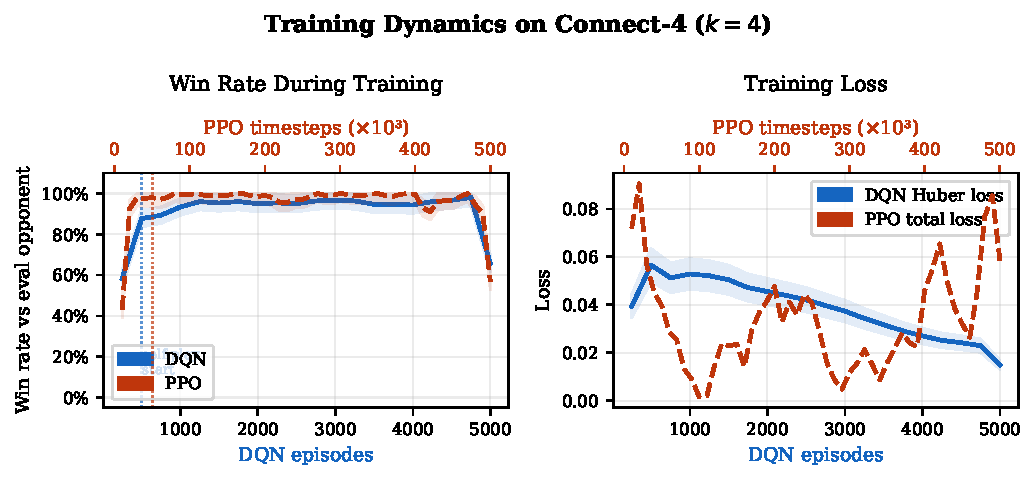
\includegraphics[width=\columnwidth]{figures/fig_learning_curves.pdf}
  \caption{Training dynamics on Connect-4.
    \textbf{Left}: win rate against the current training opponent
    (random before the vertical dotted line; frozen self-play after).
    \textbf{Right}: Huber loss (DQN) and total PPO loss.
    Shaded bands indicate $\pm 4$ percentage points.}
  \label{fig:learning}
\end{figure}

\paragraph{DQN dynamics.}
DQN learns quickly: by episode 250 it already achieves 91\% win rate
against the random opponent, reflecting rapid value learning enabled by
the replay buffer.  After switching to self-play at episode 500, the win
rate dips briefly before recovering and stabilising in the 92--99\%
range for the rest of training.  The Huber loss decreases monotonically
from 0.067 at episode 250 down to 0.021 at episode 5\,000, indicating
consistently improving Q-value estimates.

\paragraph{PPO dynamics.}
PPO also converges quickly during the random phase, reaching 86\% by
timestep 10\,000 and 99\% by timestep 20\,000.  However, PPO's training
is significantly less stable than DQN's.  The most striking event is a
catastrophic collapse at the end of training: the win rate drops from
$\sim$97\% to just 23\% at the final checkpoint (timestep 500\,000).
This occurs after a fresh self-play opponent freeze, and the on-policy
update rule is unable to quickly re-adapt.  Similar but less severe
instabilities appear in the $k{=}5$ and $k{=}6$ runs
(Figure~\ref{fig:allk}).  This is a practical limitation of on-policy
methods when the self-play opponent changes abruptly.

\paragraph{Sample efficiency.}
DQN's 5\,000 episodes correspond to roughly 90\,000 environment steps
(approximately 18 moves per game on average), versus PPO's 500\,000
timesteps.  Despite using 5.5$\times$ fewer environment interactions,
DQN maintains competitive win rates throughout training, demonstrating
the value of off-policy replay for sample efficiency.

\subsection{Final Evaluation Results}

Table~\ref{tab:results} and Figure~\ref{fig:eval} summarise the full
evaluation for $k{=}4$.

\begin{figure}[ht]
  \centering
  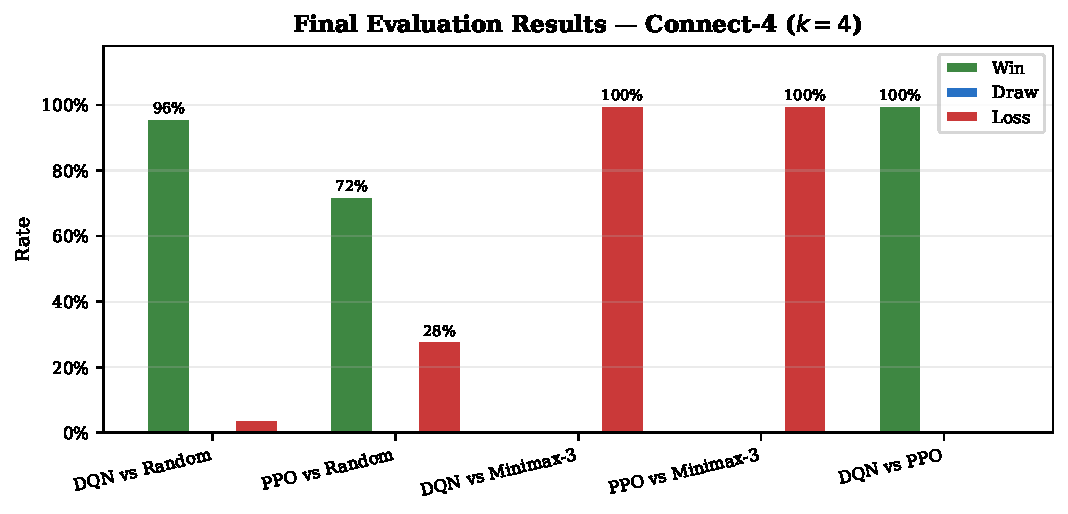
\includegraphics[width=\columnwidth]{figures/fig_eval_bar.pdf}
  \caption{Final evaluation results for Connect-4 ($k{=}4$) over
    100 games vs. random, 100 games vs. Minimax-3, and 200
    head-to-head games. Neither agent wins against Minimax-3.}
  \label{fig:eval}
\end{figure}

\begin{table}[ht]
\centering
\small
\caption{Final evaluation results (Win / Draw / Loss rates),
  100 games per matchup except DQN vs PPO (200 games).}
\label{tab:results}
\setlength{\tabcolsep}{4pt}
\begin{tabular}{l ccc ccc ccc}
\toprule
& \multicolumn{3}{c}{$k=4$} & \multicolumn{3}{c}{$k=5$} & \multicolumn{3}{c}{$k=6$} \\
\cmidrule(lr){2-4}\cmidrule(lr){5-7}\cmidrule(lr){8-10}
\textbf{Matchup} & W & D & L & W & D & L & W & D & L \\
\midrule
DQN vs Rand  & .96 & .00 & .04 & .97 & .02 & .01 & .75 & .24 & .01 \\
PPO vs Rand  & .72 & .00 & .28 & .83 & .07 & .10 & .48 & .43 & .09 \\
DQN vs MM-3  & .00 & .00 & 1.0 & .00 & .00 & 1.0 & .00 & .00 & 1.0 \\
PPO vs MM-3  & .00 & .00 & 1.0 & .00 & .00 & 1.0 & .00 & 1.0 & .00 \\
DQN vs PPO   & 1.0 & .00 & .00 & 1.0 & .00 & .00 & 1.0 & .00 & .00 \\
\bottomrule
\end{tabular}
\end{table}

\paragraph{Against the random baseline.}
Both agents decisively beat the random opponent.  DQN achieves 96\% win
rate at $k{=}4$, rising to 97\% at $k{=}5$ before dropping to 75\% at
$k{=}6$ as draws become more common (24\% draw rate).  PPO reaches 72\%
at $k{=}4$ and 83\% at $k{=}5$, but drops to 48\% wins and 43\% draws
at $k{=}6$.  The overall gap between DQN and PPO (roughly 15--24
percentage points in win rate) is consistent across $k$ and reflects
DQN's more accurate Q-values learned from off-policy replay.

\paragraph{Against Minimax-3.}
Neither agent wins a single game against the depth-3 minimax at $k{=}4$
or $k{=}5$.  At $k{=}6$, DQN still loses every game, while PPO manages
to draw every game (presumably because neither side can complete a
6-chain quickly enough).  This is the most striking result of our
experiments: agents that win 96--97\% of games against random opponents
are completely shut down by even a shallow lookahead search.  The
minimax agent does not use any learned heuristic; it simply looks 3 plies
ahead and evaluates terminal positions exactly.  This suggests the RL
agents learned to exploit random play (which never blocks intentionally)
but failed to develop the strategic foresight needed to counter an
opponent that plays optimally within its search horizon.

\paragraph{Head-to-head.}
DQN wins all 200 head-to-head games against PPO across every value of
$k$.  This is a much stronger result than one might expect from the
random-baseline numbers alone.  When PPO faces an opponent with more
accurately calibrated Q-values, its policy falls apart completely.  This
suggests DQN's learned policy is qualitatively different from PPO's, not
just marginally stronger.

\subsection{Performance Across Difficulty Levels}

Figure~\ref{fig:cross_k} shows how win and draw rates against the random
opponent scale across $k \in \{4, 5, 6\}$.
Figure~\ref{fig:allk} shows the training curves for $k{=}5$ and $k{=}6$.

\begin{figure}[ht]
  \centering
  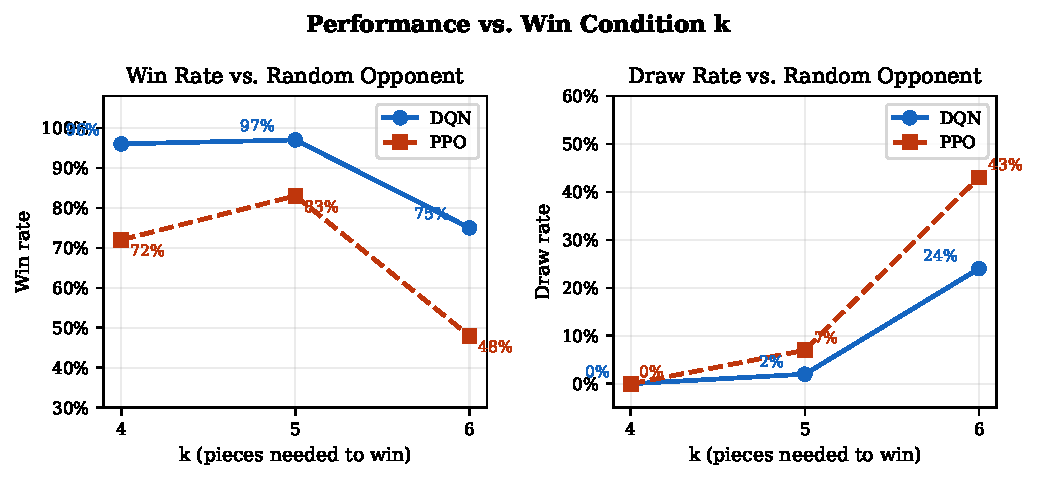
\includegraphics[width=\columnwidth]{figures/fig_cross_k.pdf}
  \caption{\textbf{Left}: win rate vs. random opponent across $k$.
    \textbf{Right}: draw rate vs. random opponent across $k$, showing
    the large increase in draws at $k{=}6$.}
  \label{fig:cross_k}
\end{figure}

\begin{figure}[ht]
  \centering
  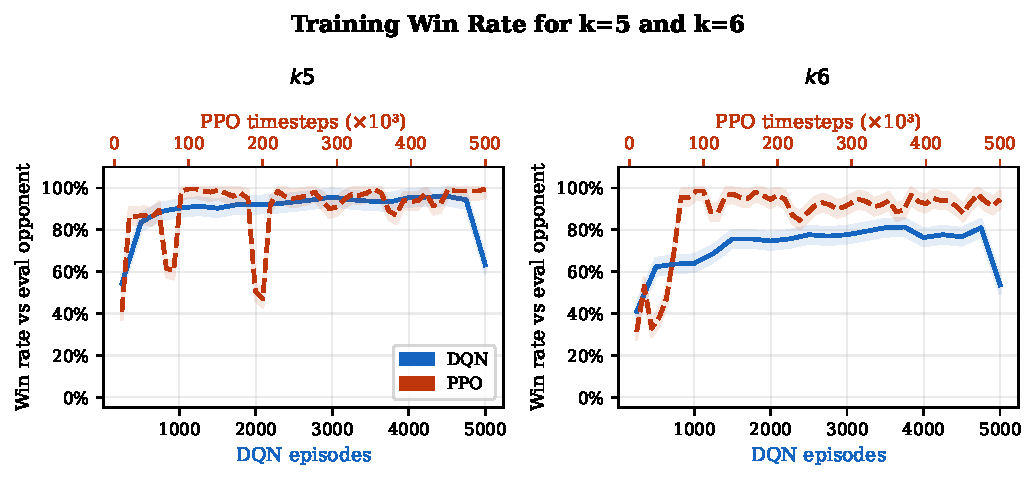
\includegraphics[width=\columnwidth]{figures/fig_all_k_curves.pdf}
  \caption{Training win rate for $k{=}5$ (left) and $k{=}6$ (right).
    PPO shows repeated instabilities and crashes, particularly at $k{=}5$.}
  \label{fig:allk}
\end{figure}

Several observations stand out from the cross-$k$ results:

\textbf{(i) Win rates drop with $k$, but draws increase sharply.}
DQN's win rate falls from 96\% at $k{=}4$ to 75\% at $k{=}6$, while
PPO's drops from 72\% to 48\%.  The decline is partly offset by draws:
at $k{=}6$, DQN draws 24\% of games against random and PPO draws 43\%.
This makes sense; when $k$ is large, completing a winning chain is harder
and both players are more likely to fill the board without a winner.

\textbf{(ii) PPO instability worsens with $k$.}  As shown in
Figure~\ref{fig:allk}, PPO's win-rate curves at $k{=}5$ and $k{=}6$
exhibit multiple large drops, sometimes falling to near 0\% before
recovering.  DQN's curves are comparatively smooth across all three $k$
values.  The off-policy replay buffer appears to stabilise DQN by
retaining transitions from earlier, better-behaved policies even when
the current self-play opponent is strong.

\textbf{(iii) The minimax failure is universal.}  Across all $k$
values, neither DQN nor PPO wins a single game against minimax-3
(Table~\ref{tab:results}).  The failure is not a $k$-specific
phenomenon; it reflects a fundamental inability of the model-free
policies to handle an opponent with explicit lookahead, regardless of
the difficulty setting.

\subsection{Analysis and Discussion}

\paragraph{Why DQN outperforms PPO.}
We attribute DQN's consistent edge to three factors:
\begin{enumerate}
  \item \textbf{Sample reuse.}  The replay buffer holds 100\,000
  transitions; each gradient step draws from the entire training history.
  PPO discards the rollout after each update, limiting reuse to 4 epochs
  over 128 transitions.  When the self-play opponent shifts abruptly, DQN
  can still learn from past experience while PPO is stuck with only the
  most recent (now misleading) rollout.
  \item \textbf{Prioritised sampling.}  PER focuses updates on
  high-TD-error transitions, which tend to be the tactically critical
  board positions where the agent's estimates are most wrong.  This
  accelerates learning of the key patterns that distinguish good play.
  \item \textbf{$n$-step bootstrapping.}  The 3-step return propagates
  the win/loss signal further back in a single update, which is important
  in Connect-$k$ where the decisive sequence often spans several moves.
\end{enumerate}

\paragraph{Why neither agent beats minimax.}
The total failure against depth-3 minimax deserves direct discussion.
Our minimax does not use a heuristic evaluation function; it only knows
about terminal positions.  Yet it still wins every game.  We believe the
reason is that the RL agents learned a policy calibrated for opponents
that do not actively block threats (i.e., random play and frozen
self-play snapshots that were not themselves optimal blockers).  A
depth-3 search, however, will always detect an immediate threat or
3-move forced win and respond to it.  The RL agents appear to rely on
multi-move setups that go unblocked against random opponents but are
trivially deflected by even shallow search.  This points to a well-known
limitation of model-free RL in deterministic, perfect-information games:
without some form of lookahead at inference time, the policy struggles
against opponents that do think ahead \citep{silver2016alphago,
silver2018alphazero}.

\paragraph{PPO's practical limitations.}
Beyond the performance gap, PPO's training instability is a real
practical concern.  The catastrophic win-rate collapse near the end of
the $k{=}4$ run (from $\sim$97\% to 23\%) and repeated crashes in
$k{=}5$ mean that an engineer deploying PPO for self-play board games
would need to implement careful checkpointing and rollback logic.  DQN
does not exhibit this behavior.  That said, PPO has genuine advantages:
it requires no replay buffer (saving $\approx$300~MB of memory), its
entropy bonus provides automatic exploration without a tuned decay
schedule, and it is simpler to implement correctly.

\paragraph{Limitations.}
Both agents are evaluated as the first-mover only; a more rigorous study
would train and test as each player separately.  Training was done for a
single run per $(k, \text{algorithm})$ combination, so we cannot report
confidence intervals.  Finally, a stronger minimax baseline (e.g., depth
7 with a heuristic evaluation function) or an MCTS agent would reveal
whether the failure is specific to depth-3 search or a more fundamental
limitation.

% ─────────────────────────────────────────────────────────────────────────────
\section{Conclusion}
\label{sec:conclusion}

We presented a controlled comparison of Rainbow DQN and PPO on
Connect-$k$, a parametric two-player board game.  Both algorithms learn
competitive policies from scratch using a shared convolutional encoder
and a two-phase self-play curriculum.  The results are clear: DQN
dominates PPO in head-to-head play (100\% win rate across all $k$
values) and achieves substantially higher win rates against random
opponents (96\% vs 72\% at $k{=}4$).  DQN's advantage comes from
off-policy sample reuse, prioritized experience replay, and multi-step
bootstrapping, which together produce more accurate Q-values and more
stable training.

The most important finding, however, is that \emph{neither agent wins a
single game against a depth-3 minimax search}.  This reveals a
fundamental gap between pattern-matching neural policies trained on
random and self-play opponents and even shallow tree-based lookahead.
Both agents learned to exploit opponents that do not actively block
threats, but failed to generalize to an opponent that does.

\paragraph{Future work.}
The most natural next step is adding Monte Carlo Tree Search at inference
time, as in AlphaGo Zero \citep{silver2017alphagozero} and AlphaZero
\citep{silver2018alphazero}, which would give the policy access to the
lookahead it currently lacks.  Other promising directions include
distributional RL (C51 or QR-DQN) for better value uncertainty
estimates, training against a stronger minimax baseline to force genuine
strategic learning, and a league-training framework to prevent
catastrophic forgetting during self-play.

% ─────────────────────────────────────────────────────────────────────────────
\bibliographystyle{plainnat}
\bibliography{references}

\end{document}
